\section{Render\-Iv  Class Reference}
\label{classRenderIv}\index{RenderIv@{Render\-Iv}}
Perform 3D rendering using the Open\-Inventor library. 


{\tt \#include $<$renderiv.h$>$}

Inheritance diagram for Render\-Iv::\begin{figure}[H]
\begin{center}
\leavevmode
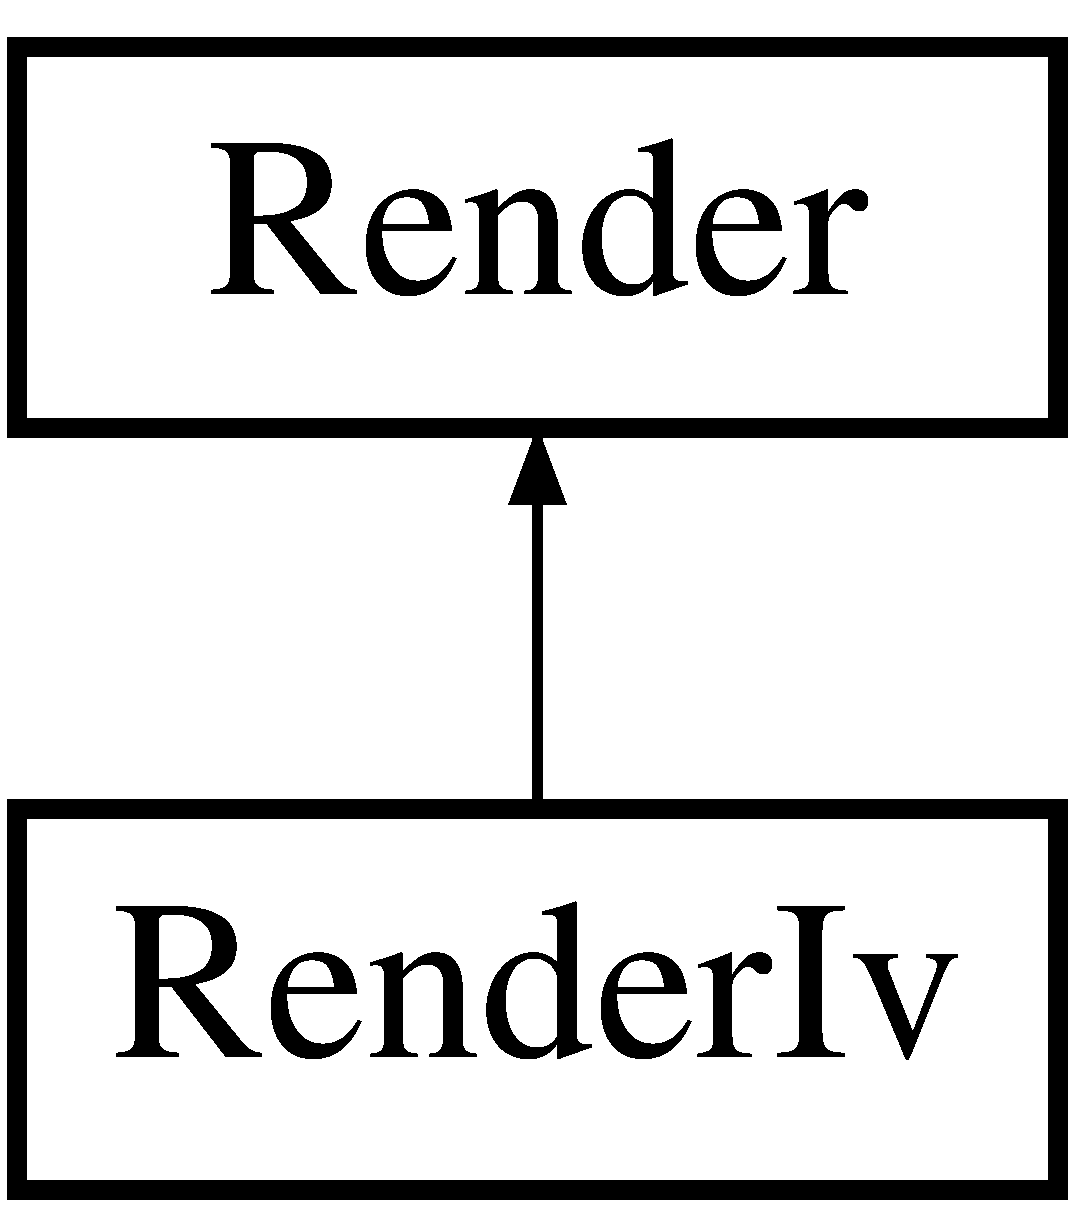
\includegraphics[height=2cm]{classRenderIv}
\end{center}
\end{figure}
\subsection*{Public Methods}
\begin{CompactItemize}
\item 
{\bf Render\-Iv} ()
\item 
{\bf Render\-Iv} (string filepath)
\item 
{\bf Render\-Iv} ({\bf Scene} $\ast$s, string filepath)
\item 
virtual {\bf $\sim$Render\-Iv} ()
\item 
virtual void {\bf Reset} ()
\begin{CompactList}\small\item\em Reset the renderer.\item\end{CompactList}\item 
virtual void {\bf Init} ()
\begin{CompactList}\small\item\em Initialized the renderer.\item\end{CompactList}\item 
virtual void {\bf Main\-Loop} ({\bf Gui} $\ast$g)
\begin{CompactList}\small\item\em If Control\-Freak = true, then Main\-Loop is entered here.\item\end{CompactList}\end{CompactItemize}
\subsection*{Protected Methods}
\begin{CompactItemize}
\item 
void {\bf \_\-Idle\-Function} ()
\item 
So\-Separator $\ast$ {\bf \_\-Read\-Iv\-File} (const char $\ast$filename)
\item 
So\-Separator $\ast$ {\bf \_\-Init\-Object} (const string \&fname)
\item 
bool {\bf \_\-Init\-Bounds\-Display} ()
\item 
bool {\bf \_\-Init\-Path\-Display} ()
\item 
So\-Separator $\ast$ {\bf \_\-Init\-Triangle\-Geom} (list$<$ {\bf MSLTriangle} $>$ \&triangles)
\item 
bool {\bf \_\-Init\-Data} ()
\item 
void {\bf \_\-Set\-Switch} (So\-Switch $\ast$p\-Switch, bool b\-Flag)
\item 
void {\bf \_\-Update\-Path\-Display} ()
\item 
void {\bf \_\-Set\-Transform} (So\-Transform $\ast$p\-Trans, double tx, double ty, double tz, double rx, double ry, double rz)
\item 
void {\bf \_\-Update\-Bodies} (const {\bf MSLVector} \&q\-Config)
\end{CompactItemize}
\subsection*{Static Protected Methods}
\begin{CompactItemize}
\item 
void {\bf \_\-Timer\-CB} (void $\ast$user\-Data, So\-Sensor $\ast$)
\end{CompactItemize}
\subsection*{Protected Attributes}
\begin{CompactItemize}
\item 
So\-Xt\-Examiner\-Viewer $\ast$ {\bf \_\-viewer}
\item 
{\bf Gui} $\ast$ {\bf \_\-p\-Gui}
\item 
So\-Separator $\ast$ {\bf \_\-iv\-Root}
\item 
So\-Separator $\ast$ {\bf \_\-iv\-Data}
\item 
So\-Switch $\ast$ {\bf \_\-iv\-Bounds\-Switch}
\item 
bool {\bf \_\-b\-Display\-Bounds}
\item 
So\-Switch $\ast$ {\bf \_\-iv\-Path\-Switch}
\item 
So\-Vertex\-Property $\ast$ {\bf \_\-p\-Path\-Vertex\-Prop}
\item 
int {\bf \_\-path\-Frames}
\item 
bool {\bf \_\-b\-Display\-Path}
\item 
list$<$ So\-Transform $\ast$ $>$ {\bf \_\-body\-Trans}
\item 
int {\bf cam\-Toggle}
\item 
bool {\bf \_\-b\-Attached\-Camera}
\item 
So\-Switch $\ast$ {\bf Cam\-Switch}
\item 
So\-Perspective\-Camera $\ast$ {\bf def\-Cam}
\item 
So\-Perspective\-Camera $\ast$ {\bf attached\-Cam}
\item 
So\-Point\-Light $\ast$ {\bf light\-Source}
\item 
float {\bf \_\-iv\-Position} [3]
\item 
float {\bf \_\-iv\-Orientation} [3]
\item 
float {\bf \_\-iv\-Bounding\-Box\-Min} [3]
\item 
float {\bf \_\-iv\-Bounding\-Box\-Max} [3]
\item 
float {\bf \_\-iv\-Scene\-Center} [3]
\item 
float {\bf Cam\-Pos\-X}
\item 
float {\bf Cam\-Pos\-Y}
\item 
float {\bf Cam\-Pos\-Z}
\item 
float {\bf Cam\-View\-X}
\item 
float {\bf Cam\-View\-Y}
\item 
float {\bf Cam\-View\-Z}
\item 
float {\bf \_\-iv\-View\-Length}
\item 
float {\bf \_\-iv\-Focal\-Dist}
\item 
float {\bf \_\-iv\-Near\-Dist}
\item 
float {\bf \_\-iv\-Far\-Dist}
\item 
float {\bf Light\-Pos\-X}
\item 
float {\bf Light\-Pos\-Y}
\item 
float {\bf Light\-Pos\-Z}
\item 
float {\bf Cam\-Up\-X}
\item 
float {\bf Cam\-Up\-Y}
\item 
float {\bf Cam\-Up\-Z}
\item 
bool {\bf \_\-b\-Multiple\-Views}
\item 
So\-Separator $\ast$ {\bf \_\-iv\-Top\-Left\-Object}
\item 
So\-Separator $\ast$ {\bf \_\-iv\-Top\-Right\-Object}
\item 
So\-Separator $\ast$ {\bf \_\-iv\-Bottom\-Left\-Object}
\item 
So\-Separator $\ast$ {\bf \_\-iv\-Bottom\-Right\-Object}
\item 
int {\bf Multiple\-Views\-Toggle}
\item 
So\-Xt\-Examiner\-Viewer $\ast$ {\bf Top\-Left\-Viewer}
\item 
So\-Xt\-Examiner\-Viewer $\ast$ {\bf Top\-Right\-Viewer}
\item 
So\-Xt\-Examiner\-Viewer $\ast$ {\bf Bottom\-Left\-Viewer}
\item 
So\-Xt\-Examiner\-Viewer $\ast$ {\bf Bottom\-Right\-Viewer}
\item 
Widget {\bf main\-Window}
\item 
So\-Orthographic\-Camera $\ast$ {\bf Top\-Left\-Camera}
\item 
So\-Orthographic\-Camera $\ast$ {\bf Top\-Right\-Camera}
\item 
So\-Orthographic\-Camera $\ast$ {\bf Bottom\-Left\-Camera}
\item 
So\-Perspective\-Camera $\ast$ {\bf Bottom\-Right\-Camera}
\end{CompactItemize}


\subsection{Detailed Description}
Perform 3D rendering using the Open\-Inventor library.



\subsection{Constructor \& Destructor Documentation}
\index{RenderIv@{Render\-Iv}!RenderIv@{RenderIv}}
\index{RenderIv@{RenderIv}!RenderIv@{Render\-Iv}}
\subsubsection{\setlength{\rightskip}{0pt plus 5cm}Render\-Iv::Render\-Iv ()}\label{classRenderIv_a0}


\index{RenderIv@{Render\-Iv}!RenderIv@{RenderIv}}
\index{RenderIv@{RenderIv}!RenderIv@{Render\-Iv}}
\subsubsection{\setlength{\rightskip}{0pt plus 5cm}Render\-Iv::Render\-Iv (string {\em filepath})}\label{classRenderIv_a1}


\index{RenderIv@{Render\-Iv}!RenderIv@{RenderIv}}
\index{RenderIv@{RenderIv}!RenderIv@{Render\-Iv}}
\subsubsection{\setlength{\rightskip}{0pt plus 5cm}Render\-Iv::Render\-Iv ({\bf Scene} $\ast$ {\em s}, string {\em filepath})}\label{classRenderIv_a2}


\index{RenderIv@{Render\-Iv}!~RenderIv@{$\sim$RenderIv}}
\index{~RenderIv@{$\sim$RenderIv}!RenderIv@{Render\-Iv}}
\subsubsection{\setlength{\rightskip}{0pt plus 5cm}Render\-Iv::$\sim$Render\-Iv ()\hspace{0.3cm}{\tt  [virtual]}}\label{classRenderIv_a3}




\subsection{Member Function Documentation}
\index{RenderIv@{Render\-Iv}!_IdleFunction@{\_\-IdleFunction}}
\index{_IdleFunction@{\_\-IdleFunction}!RenderIv@{Render\-Iv}}
\subsubsection{\setlength{\rightskip}{0pt plus 5cm}void Render\-Iv::\_\-Idle\-Function ()\hspace{0.3cm}{\tt  [inline, protected]}}\label{classRenderIv_b0}


\index{RenderIv@{Render\-Iv}!_InitBoundsDisplay@{\_\-InitBoundsDisplay}}
\index{_InitBoundsDisplay@{\_\-InitBoundsDisplay}!RenderIv@{Render\-Iv}}
\subsubsection{\setlength{\rightskip}{0pt plus 5cm}bool Render\-Iv::\_\-Init\-Bounds\-Display ()\hspace{0.3cm}{\tt  [protected]}}\label{classRenderIv_b3}


\index{RenderIv@{Render\-Iv}!_InitData@{\_\-InitData}}
\index{_InitData@{\_\-InitData}!RenderIv@{Render\-Iv}}
\subsubsection{\setlength{\rightskip}{0pt plus 5cm}bool Render\-Iv::\_\-Init\-Data ()\hspace{0.3cm}{\tt  [protected]}}\label{classRenderIv_b6}


\index{RenderIv@{Render\-Iv}!_InitObject@{\_\-InitObject}}
\index{_InitObject@{\_\-InitObject}!RenderIv@{Render\-Iv}}
\subsubsection{\setlength{\rightskip}{0pt plus 5cm}So\-Separator $\ast$ Render\-Iv::\_\-Init\-Object (const string \& {\em fname})\hspace{0.3cm}{\tt  [protected]}}\label{classRenderIv_b2}


\index{RenderIv@{Render\-Iv}!_InitPathDisplay@{\_\-InitPathDisplay}}
\index{_InitPathDisplay@{\_\-InitPathDisplay}!RenderIv@{Render\-Iv}}
\subsubsection{\setlength{\rightskip}{0pt plus 5cm}bool Render\-Iv::\_\-Init\-Path\-Display ()\hspace{0.3cm}{\tt  [protected]}}\label{classRenderIv_b4}


\index{RenderIv@{Render\-Iv}!_InitTriangleGeom@{\_\-InitTriangleGeom}}
\index{_InitTriangleGeom@{\_\-InitTriangleGeom}!RenderIv@{Render\-Iv}}
\subsubsection{\setlength{\rightskip}{0pt plus 5cm}So\-Separator $\ast$ Render\-Iv::\_\-Init\-Triangle\-Geom (list$<$ {\bf MSLTriangle} $>$ \& {\em triangles})\hspace{0.3cm}{\tt  [protected]}}\label{classRenderIv_b5}


\index{RenderIv@{Render\-Iv}!_ReadIvFile@{\_\-ReadIvFile}}
\index{_ReadIvFile@{\_\-ReadIvFile}!RenderIv@{Render\-Iv}}
\subsubsection{\setlength{\rightskip}{0pt plus 5cm}So\-Separator $\ast$ Render\-Iv::\_\-Read\-Iv\-File (const char $\ast$ {\em filename})\hspace{0.3cm}{\tt  [protected]}}\label{classRenderIv_b1}


\index{RenderIv@{Render\-Iv}!_SetSwitch@{\_\-SetSwitch}}
\index{_SetSwitch@{\_\-SetSwitch}!RenderIv@{Render\-Iv}}
\subsubsection{\setlength{\rightskip}{0pt plus 5cm}void Render\-Iv::\_\-Set\-Switch (So\-Switch $\ast$ {\em p\-Switch}, bool {\em b\-Flag})\hspace{0.3cm}{\tt  [inline, protected]}}\label{classRenderIv_b7}


\index{RenderIv@{Render\-Iv}!_SetTransform@{\_\-SetTransform}}
\index{_SetTransform@{\_\-SetTransform}!RenderIv@{Render\-Iv}}
\subsubsection{\setlength{\rightskip}{0pt plus 5cm}void Render\-Iv::\_\-Set\-Transform (So\-Transform $\ast$ {\em p\-Trans}, double {\em tx}, double {\em ty}, double {\em tz}, double {\em rx}, double {\em ry}, double {\em rz})\hspace{0.3cm}{\tt  [inline, protected]}}\label{classRenderIv_b9}


\index{RenderIv@{Render\-Iv}!_TimerCB@{\_\-TimerCB}}
\index{_TimerCB@{\_\-TimerCB}!RenderIv@{Render\-Iv}}
\subsubsection{\setlength{\rightskip}{0pt plus 5cm}void Render\-Iv::\_\-Timer\-CB (void $\ast$ {\em user\-Data}, So\-Sensor $\ast$)\hspace{0.3cm}{\tt  [static, protected]}}\label{classRenderIv_e0}


\index{RenderIv@{Render\-Iv}!_UpdateBodies@{\_\-UpdateBodies}}
\index{_UpdateBodies@{\_\-UpdateBodies}!RenderIv@{Render\-Iv}}
\subsubsection{\setlength{\rightskip}{0pt plus 5cm}void Render\-Iv::\_\-Update\-Bodies (const {\bf MSLVector} \& {\em q\-Config})\hspace{0.3cm}{\tt  [inline, protected]}}\label{classRenderIv_b10}


\index{RenderIv@{Render\-Iv}!_UpdatePathDisplay@{\_\-UpdatePathDisplay}}
\index{_UpdatePathDisplay@{\_\-UpdatePathDisplay}!RenderIv@{Render\-Iv}}
\subsubsection{\setlength{\rightskip}{0pt plus 5cm}void Render\-Iv::\_\-Update\-Path\-Display ()\hspace{0.3cm}{\tt  [inline, protected]}}\label{classRenderIv_b8}


\index{RenderIv@{Render\-Iv}!Init@{Init}}
\index{Init@{Init}!RenderIv@{Render\-Iv}}
\subsubsection{\setlength{\rightskip}{0pt plus 5cm}void Render\-Iv::Init ()\hspace{0.3cm}{\tt  [virtual]}}\label{classRenderIv_a5}


Initialized the renderer.



Reimplemented from {\bf Render} {\rm (p.\,\pageref{classRender_a4})}.\index{RenderIv@{Render\-Iv}!MainLoop@{MainLoop}}
\index{MainLoop@{MainLoop}!RenderIv@{Render\-Iv}}
\subsubsection{\setlength{\rightskip}{0pt plus 5cm}void Render\-Iv::Main\-Loop ({\bf Gui} $\ast$ {\em g})\hspace{0.3cm}{\tt  [virtual]}}\label{classRenderIv_a6}


If Control\-Freak = true, then Main\-Loop is entered here.



Reimplemented from {\bf Render} {\rm (p.\,\pageref{classRender_a6})}.\index{RenderIv@{Render\-Iv}!Reset@{Reset}}
\index{Reset@{Reset}!RenderIv@{Render\-Iv}}
\subsubsection{\setlength{\rightskip}{0pt plus 5cm}void Render\-Iv::Reset ()\hspace{0.3cm}{\tt  [virtual]}}\label{classRenderIv_a4}


Reset the renderer.



Reimplemented from {\bf Render} {\rm (p.\,\pageref{classRender_a7})}.

\subsection{Member Data Documentation}
\index{RenderIv@{Render\-Iv}!_bAttachedCamera@{\_\-bAttachedCamera}}
\index{_bAttachedCamera@{\_\-bAttachedCamera}!RenderIv@{Render\-Iv}}
\subsubsection{\setlength{\rightskip}{0pt plus 5cm}bool Render\-Iv::\_\-b\-Attached\-Camera\hspace{0.3cm}{\tt  [protected]}}\label{classRenderIv_n12}


\index{RenderIv@{Render\-Iv}!_bDisplayBounds@{\_\-bDisplayBounds}}
\index{_bDisplayBounds@{\_\-bDisplayBounds}!RenderIv@{Render\-Iv}}
\subsubsection{\setlength{\rightskip}{0pt plus 5cm}bool Render\-Iv::\_\-b\-Display\-Bounds\hspace{0.3cm}{\tt  [protected]}}\label{classRenderIv_n5}


\index{RenderIv@{Render\-Iv}!_bDisplayPath@{\_\-bDisplayPath}}
\index{_bDisplayPath@{\_\-bDisplayPath}!RenderIv@{Render\-Iv}}
\subsubsection{\setlength{\rightskip}{0pt plus 5cm}bool Render\-Iv::\_\-b\-Display\-Path\hspace{0.3cm}{\tt  [protected]}}\label{classRenderIv_n9}


\index{RenderIv@{Render\-Iv}!_bMultipleViews@{\_\-bMultipleViews}}
\index{_bMultipleViews@{\_\-bMultipleViews}!RenderIv@{Render\-Iv}}
\subsubsection{\setlength{\rightskip}{0pt plus 5cm}bool Render\-Iv::\_\-b\-Multiple\-Views\hspace{0.3cm}{\tt  [protected]}}\label{classRenderIv_n38}


\index{RenderIv@{Render\-Iv}!_bodyTrans@{\_\-bodyTrans}}
\index{_bodyTrans@{\_\-bodyTrans}!RenderIv@{Render\-Iv}}
\subsubsection{\setlength{\rightskip}{0pt plus 5cm}list$<$So\-Transform$\ast$$>$ Render\-Iv::\_\-body\-Trans\hspace{0.3cm}{\tt  [protected]}}\label{classRenderIv_n10}


\index{RenderIv@{Render\-Iv}!_ivBottomLeftObject@{\_\-ivBottomLeftObject}}
\index{_ivBottomLeftObject@{\_\-ivBottomLeftObject}!RenderIv@{Render\-Iv}}
\subsubsection{\setlength{\rightskip}{0pt plus 5cm}So\-Separator$\ast$ Render\-Iv::\_\-iv\-Bottom\-Left\-Object\hspace{0.3cm}{\tt  [protected]}}\label{classRenderIv_n41}


\index{RenderIv@{Render\-Iv}!_ivBottomRightObject@{\_\-ivBottomRightObject}}
\index{_ivBottomRightObject@{\_\-ivBottomRightObject}!RenderIv@{Render\-Iv}}
\subsubsection{\setlength{\rightskip}{0pt plus 5cm}So\-Separator$\ast$ Render\-Iv::\_\-iv\-Bottom\-Right\-Object\hspace{0.3cm}{\tt  [protected]}}\label{classRenderIv_n42}


\index{RenderIv@{Render\-Iv}!_ivBoundingBoxMax@{\_\-ivBoundingBoxMax}}
\index{_ivBoundingBoxMax@{\_\-ivBoundingBoxMax}!RenderIv@{Render\-Iv}}
\subsubsection{\setlength{\rightskip}{0pt plus 5cm}float Render\-Iv::\_\-iv\-Bounding\-Box\-Max[3]\hspace{0.3cm}{\tt  [protected]}}\label{classRenderIv_n20}


\index{RenderIv@{Render\-Iv}!_ivBoundingBoxMin@{\_\-ivBoundingBoxMin}}
\index{_ivBoundingBoxMin@{\_\-ivBoundingBoxMin}!RenderIv@{Render\-Iv}}
\subsubsection{\setlength{\rightskip}{0pt plus 5cm}float Render\-Iv::\_\-iv\-Bounding\-Box\-Min[3]\hspace{0.3cm}{\tt  [protected]}}\label{classRenderIv_n19}


\index{RenderIv@{Render\-Iv}!_ivBoundsSwitch@{\_\-ivBoundsSwitch}}
\index{_ivBoundsSwitch@{\_\-ivBoundsSwitch}!RenderIv@{Render\-Iv}}
\subsubsection{\setlength{\rightskip}{0pt plus 5cm}So\-Switch$\ast$ Render\-Iv::\_\-iv\-Bounds\-Switch\hspace{0.3cm}{\tt  [protected]}}\label{classRenderIv_n4}


\index{RenderIv@{Render\-Iv}!_ivData@{\_\-ivData}}
\index{_ivData@{\_\-ivData}!RenderIv@{Render\-Iv}}
\subsubsection{\setlength{\rightskip}{0pt plus 5cm}So\-Separator$\ast$ Render\-Iv::\_\-iv\-Data\hspace{0.3cm}{\tt  [protected]}}\label{classRenderIv_n3}


\index{RenderIv@{Render\-Iv}!_ivFarDist@{\_\-ivFarDist}}
\index{_ivFarDist@{\_\-ivFarDist}!RenderIv@{Render\-Iv}}
\subsubsection{\setlength{\rightskip}{0pt plus 5cm}float Render\-Iv::\_\-iv\-Far\-Dist\hspace{0.3cm}{\tt  [protected]}}\label{classRenderIv_n31}


\index{RenderIv@{Render\-Iv}!_ivFocalDist@{\_\-ivFocalDist}}
\index{_ivFocalDist@{\_\-ivFocalDist}!RenderIv@{Render\-Iv}}
\subsubsection{\setlength{\rightskip}{0pt plus 5cm}float Render\-Iv::\_\-iv\-Focal\-Dist\hspace{0.3cm}{\tt  [protected]}}\label{classRenderIv_n29}


\index{RenderIv@{Render\-Iv}!_ivNearDist@{\_\-ivNearDist}}
\index{_ivNearDist@{\_\-ivNearDist}!RenderIv@{Render\-Iv}}
\subsubsection{\setlength{\rightskip}{0pt plus 5cm}float Render\-Iv::\_\-iv\-Near\-Dist\hspace{0.3cm}{\tt  [protected]}}\label{classRenderIv_n30}


\index{RenderIv@{Render\-Iv}!_ivOrientation@{\_\-ivOrientation}}
\index{_ivOrientation@{\_\-ivOrientation}!RenderIv@{Render\-Iv}}
\subsubsection{\setlength{\rightskip}{0pt plus 5cm}float Render\-Iv::\_\-iv\-Orientation[3]\hspace{0.3cm}{\tt  [protected]}}\label{classRenderIv_n18}


\index{RenderIv@{Render\-Iv}!_ivPathSwitch@{\_\-ivPathSwitch}}
\index{_ivPathSwitch@{\_\-ivPathSwitch}!RenderIv@{Render\-Iv}}
\subsubsection{\setlength{\rightskip}{0pt plus 5cm}So\-Switch$\ast$ Render\-Iv::\_\-iv\-Path\-Switch\hspace{0.3cm}{\tt  [protected]}}\label{classRenderIv_n6}


\index{RenderIv@{Render\-Iv}!_ivPosition@{\_\-ivPosition}}
\index{_ivPosition@{\_\-ivPosition}!RenderIv@{Render\-Iv}}
\subsubsection{\setlength{\rightskip}{0pt plus 5cm}float Render\-Iv::\_\-iv\-Position[3]\hspace{0.3cm}{\tt  [protected]}}\label{classRenderIv_n17}


\index{RenderIv@{Render\-Iv}!_ivRoot@{\_\-ivRoot}}
\index{_ivRoot@{\_\-ivRoot}!RenderIv@{Render\-Iv}}
\subsubsection{\setlength{\rightskip}{0pt plus 5cm}So\-Separator$\ast$ Render\-Iv::\_\-iv\-Root\hspace{0.3cm}{\tt  [protected]}}\label{classRenderIv_n2}


\index{RenderIv@{Render\-Iv}!_ivSceneCenter@{\_\-ivSceneCenter}}
\index{_ivSceneCenter@{\_\-ivSceneCenter}!RenderIv@{Render\-Iv}}
\subsubsection{\setlength{\rightskip}{0pt plus 5cm}float Render\-Iv::\_\-iv\-Scene\-Center[3]\hspace{0.3cm}{\tt  [protected]}}\label{classRenderIv_n21}


\index{RenderIv@{Render\-Iv}!_ivTopLeftObject@{\_\-ivTopLeftObject}}
\index{_ivTopLeftObject@{\_\-ivTopLeftObject}!RenderIv@{Render\-Iv}}
\subsubsection{\setlength{\rightskip}{0pt plus 5cm}So\-Separator$\ast$ Render\-Iv::\_\-iv\-Top\-Left\-Object\hspace{0.3cm}{\tt  [protected]}}\label{classRenderIv_n39}


\index{RenderIv@{Render\-Iv}!_ivTopRightObject@{\_\-ivTopRightObject}}
\index{_ivTopRightObject@{\_\-ivTopRightObject}!RenderIv@{Render\-Iv}}
\subsubsection{\setlength{\rightskip}{0pt plus 5cm}So\-Separator$\ast$ Render\-Iv::\_\-iv\-Top\-Right\-Object\hspace{0.3cm}{\tt  [protected]}}\label{classRenderIv_n40}


\index{RenderIv@{Render\-Iv}!_ivViewLength@{\_\-ivViewLength}}
\index{_ivViewLength@{\_\-ivViewLength}!RenderIv@{Render\-Iv}}
\subsubsection{\setlength{\rightskip}{0pt plus 5cm}float Render\-Iv::\_\-iv\-View\-Length\hspace{0.3cm}{\tt  [protected]}}\label{classRenderIv_n28}


\index{RenderIv@{Render\-Iv}!_pathFrames@{\_\-pathFrames}}
\index{_pathFrames@{\_\-pathFrames}!RenderIv@{Render\-Iv}}
\subsubsection{\setlength{\rightskip}{0pt plus 5cm}int Render\-Iv::\_\-path\-Frames\hspace{0.3cm}{\tt  [protected]}}\label{classRenderIv_n8}


\index{RenderIv@{Render\-Iv}!_pGui@{\_\-pGui}}
\index{_pGui@{\_\-pGui}!RenderIv@{Render\-Iv}}
\subsubsection{\setlength{\rightskip}{0pt plus 5cm}{\bf Gui}$\ast$ Render\-Iv::\_\-p\-Gui\hspace{0.3cm}{\tt  [protected]}}\label{classRenderIv_n1}


\index{RenderIv@{Render\-Iv}!_pPathVertexProp@{\_\-pPathVertexProp}}
\index{_pPathVertexProp@{\_\-pPathVertexProp}!RenderIv@{Render\-Iv}}
\subsubsection{\setlength{\rightskip}{0pt plus 5cm}So\-Vertex\-Property$\ast$ Render\-Iv::\_\-p\-Path\-Vertex\-Prop\hspace{0.3cm}{\tt  [protected]}}\label{classRenderIv_n7}


\index{RenderIv@{Render\-Iv}!_viewer@{\_\-viewer}}
\index{_viewer@{\_\-viewer}!RenderIv@{Render\-Iv}}
\subsubsection{\setlength{\rightskip}{0pt plus 5cm}So\-Xt\-Examiner\-Viewer$\ast$ Render\-Iv::\_\-viewer\hspace{0.3cm}{\tt  [protected]}}\label{classRenderIv_n0}


\index{RenderIv@{Render\-Iv}!attachedCam@{attachedCam}}
\index{attachedCam@{attachedCam}!RenderIv@{Render\-Iv}}
\subsubsection{\setlength{\rightskip}{0pt plus 5cm}So\-Perspective\-Camera$\ast$ Render\-Iv::attached\-Cam\hspace{0.3cm}{\tt  [protected]}}\label{classRenderIv_n15}


\index{RenderIv@{Render\-Iv}!BottomLeftCamera@{BottomLeftCamera}}
\index{BottomLeftCamera@{BottomLeftCamera}!RenderIv@{Render\-Iv}}
\subsubsection{\setlength{\rightskip}{0pt plus 5cm}So\-Orthographic\-Camera$\ast$ Render\-Iv::Bottom\-Left\-Camera\hspace{0.3cm}{\tt  [protected]}}\label{classRenderIv_n51}


\index{RenderIv@{Render\-Iv}!BottomLeftViewer@{BottomLeftViewer}}
\index{BottomLeftViewer@{BottomLeftViewer}!RenderIv@{Render\-Iv}}
\subsubsection{\setlength{\rightskip}{0pt plus 5cm}So\-Xt\-Examiner\-Viewer$\ast$ Render\-Iv::Bottom\-Left\-Viewer\hspace{0.3cm}{\tt  [protected]}}\label{classRenderIv_n46}


\index{RenderIv@{Render\-Iv}!BottomRightCamera@{BottomRightCamera}}
\index{BottomRightCamera@{BottomRightCamera}!RenderIv@{Render\-Iv}}
\subsubsection{\setlength{\rightskip}{0pt plus 5cm}So\-Perspective\-Camera$\ast$ Render\-Iv::Bottom\-Right\-Camera\hspace{0.3cm}{\tt  [protected]}}\label{classRenderIv_n52}


\index{RenderIv@{Render\-Iv}!BottomRightViewer@{BottomRightViewer}}
\index{BottomRightViewer@{BottomRightViewer}!RenderIv@{Render\-Iv}}
\subsubsection{\setlength{\rightskip}{0pt plus 5cm}So\-Xt\-Examiner\-Viewer$\ast$ Render\-Iv::Bottom\-Right\-Viewer\hspace{0.3cm}{\tt  [protected]}}\label{classRenderIv_n47}


\index{RenderIv@{Render\-Iv}!CamPosX@{CamPosX}}
\index{CamPosX@{CamPosX}!RenderIv@{Render\-Iv}}
\subsubsection{\setlength{\rightskip}{0pt plus 5cm}float Render\-Iv::Cam\-Pos\-X\hspace{0.3cm}{\tt  [protected]}}\label{classRenderIv_n22}


\index{RenderIv@{Render\-Iv}!CamPosY@{CamPosY}}
\index{CamPosY@{CamPosY}!RenderIv@{Render\-Iv}}
\subsubsection{\setlength{\rightskip}{0pt plus 5cm}float Render\-Iv::Cam\-Pos\-Y\hspace{0.3cm}{\tt  [protected]}}\label{classRenderIv_n23}


\index{RenderIv@{Render\-Iv}!CamPosZ@{CamPosZ}}
\index{CamPosZ@{CamPosZ}!RenderIv@{Render\-Iv}}
\subsubsection{\setlength{\rightskip}{0pt plus 5cm}float Render\-Iv::Cam\-Pos\-Z\hspace{0.3cm}{\tt  [protected]}}\label{classRenderIv_n24}


\index{RenderIv@{Render\-Iv}!CamSwitch@{CamSwitch}}
\index{CamSwitch@{CamSwitch}!RenderIv@{Render\-Iv}}
\subsubsection{\setlength{\rightskip}{0pt plus 5cm}So\-Switch$\ast$ Render\-Iv::Cam\-Switch\hspace{0.3cm}{\tt  [protected]}}\label{classRenderIv_n13}


\index{RenderIv@{Render\-Iv}!camToggle@{camToggle}}
\index{camToggle@{camToggle}!RenderIv@{Render\-Iv}}
\subsubsection{\setlength{\rightskip}{0pt plus 5cm}int Render\-Iv::cam\-Toggle\hspace{0.3cm}{\tt  [protected]}}\label{classRenderIv_n11}


\index{RenderIv@{Render\-Iv}!CamUpX@{CamUpX}}
\index{CamUpX@{CamUpX}!RenderIv@{Render\-Iv}}
\subsubsection{\setlength{\rightskip}{0pt plus 5cm}float Render\-Iv::Cam\-Up\-X\hspace{0.3cm}{\tt  [protected]}}\label{classRenderIv_n35}


\index{RenderIv@{Render\-Iv}!CamUpY@{CamUpY}}
\index{CamUpY@{CamUpY}!RenderIv@{Render\-Iv}}
\subsubsection{\setlength{\rightskip}{0pt plus 5cm}float Render\-Iv::Cam\-Up\-Y\hspace{0.3cm}{\tt  [protected]}}\label{classRenderIv_n36}


\index{RenderIv@{Render\-Iv}!CamUpZ@{CamUpZ}}
\index{CamUpZ@{CamUpZ}!RenderIv@{Render\-Iv}}
\subsubsection{\setlength{\rightskip}{0pt plus 5cm}float Render\-Iv::Cam\-Up\-Z\hspace{0.3cm}{\tt  [protected]}}\label{classRenderIv_n37}


\index{RenderIv@{Render\-Iv}!CamViewX@{CamViewX}}
\index{CamViewX@{CamViewX}!RenderIv@{Render\-Iv}}
\subsubsection{\setlength{\rightskip}{0pt plus 5cm}float Render\-Iv::Cam\-View\-X\hspace{0.3cm}{\tt  [protected]}}\label{classRenderIv_n25}


\index{RenderIv@{Render\-Iv}!CamViewY@{CamViewY}}
\index{CamViewY@{CamViewY}!RenderIv@{Render\-Iv}}
\subsubsection{\setlength{\rightskip}{0pt plus 5cm}float Render\-Iv::Cam\-View\-Y\hspace{0.3cm}{\tt  [protected]}}\label{classRenderIv_n26}


\index{RenderIv@{Render\-Iv}!CamViewZ@{CamViewZ}}
\index{CamViewZ@{CamViewZ}!RenderIv@{Render\-Iv}}
\subsubsection{\setlength{\rightskip}{0pt plus 5cm}float Render\-Iv::Cam\-View\-Z\hspace{0.3cm}{\tt  [protected]}}\label{classRenderIv_n27}


\index{RenderIv@{Render\-Iv}!defCam@{defCam}}
\index{defCam@{defCam}!RenderIv@{Render\-Iv}}
\subsubsection{\setlength{\rightskip}{0pt plus 5cm}So\-Perspective\-Camera$\ast$ Render\-Iv::def\-Cam\hspace{0.3cm}{\tt  [protected]}}\label{classRenderIv_n14}


\index{RenderIv@{Render\-Iv}!LightPosX@{LightPosX}}
\index{LightPosX@{LightPosX}!RenderIv@{Render\-Iv}}
\subsubsection{\setlength{\rightskip}{0pt plus 5cm}float Render\-Iv::Light\-Pos\-X\hspace{0.3cm}{\tt  [protected]}}\label{classRenderIv_n32}


\index{RenderIv@{Render\-Iv}!LightPosY@{LightPosY}}
\index{LightPosY@{LightPosY}!RenderIv@{Render\-Iv}}
\subsubsection{\setlength{\rightskip}{0pt plus 5cm}float Render\-Iv::Light\-Pos\-Y\hspace{0.3cm}{\tt  [protected]}}\label{classRenderIv_n33}


\index{RenderIv@{Render\-Iv}!LightPosZ@{LightPosZ}}
\index{LightPosZ@{LightPosZ}!RenderIv@{Render\-Iv}}
\subsubsection{\setlength{\rightskip}{0pt plus 5cm}float Render\-Iv::Light\-Pos\-Z\hspace{0.3cm}{\tt  [protected]}}\label{classRenderIv_n34}


\index{RenderIv@{Render\-Iv}!lightSource@{lightSource}}
\index{lightSource@{lightSource}!RenderIv@{Render\-Iv}}
\subsubsection{\setlength{\rightskip}{0pt plus 5cm}So\-Point\-Light$\ast$ Render\-Iv::light\-Source\hspace{0.3cm}{\tt  [protected]}}\label{classRenderIv_n16}


\index{RenderIv@{Render\-Iv}!mainWindow@{mainWindow}}
\index{mainWindow@{mainWindow}!RenderIv@{Render\-Iv}}
\subsubsection{\setlength{\rightskip}{0pt plus 5cm}Widget Render\-Iv::main\-Window\hspace{0.3cm}{\tt  [protected]}}\label{classRenderIv_n48}


\index{RenderIv@{Render\-Iv}!MultipleViewsToggle@{MultipleViewsToggle}}
\index{MultipleViewsToggle@{MultipleViewsToggle}!RenderIv@{Render\-Iv}}
\subsubsection{\setlength{\rightskip}{0pt plus 5cm}int Render\-Iv::Multiple\-Views\-Toggle\hspace{0.3cm}{\tt  [protected]}}\label{classRenderIv_n43}


\index{RenderIv@{Render\-Iv}!TopLeftCamera@{TopLeftCamera}}
\index{TopLeftCamera@{TopLeftCamera}!RenderIv@{Render\-Iv}}
\subsubsection{\setlength{\rightskip}{0pt plus 5cm}So\-Orthographic\-Camera$\ast$ Render\-Iv::Top\-Left\-Camera\hspace{0.3cm}{\tt  [protected]}}\label{classRenderIv_n49}


\index{RenderIv@{Render\-Iv}!TopLeftViewer@{TopLeftViewer}}
\index{TopLeftViewer@{TopLeftViewer}!RenderIv@{Render\-Iv}}
\subsubsection{\setlength{\rightskip}{0pt plus 5cm}So\-Xt\-Examiner\-Viewer$\ast$ Render\-Iv::Top\-Left\-Viewer\hspace{0.3cm}{\tt  [protected]}}\label{classRenderIv_n44}


\index{RenderIv@{Render\-Iv}!TopRightCamera@{TopRightCamera}}
\index{TopRightCamera@{TopRightCamera}!RenderIv@{Render\-Iv}}
\subsubsection{\setlength{\rightskip}{0pt plus 5cm}So\-Orthographic\-Camera$\ast$ Render\-Iv::Top\-Right\-Camera\hspace{0.3cm}{\tt  [protected]}}\label{classRenderIv_n50}


\index{RenderIv@{Render\-Iv}!TopRightViewer@{TopRightViewer}}
\index{TopRightViewer@{TopRightViewer}!RenderIv@{Render\-Iv}}
\subsubsection{\setlength{\rightskip}{0pt plus 5cm}So\-Xt\-Examiner\-Viewer$\ast$ Render\-Iv::Top\-Right\-Viewer\hspace{0.3cm}{\tt  [protected]}}\label{classRenderIv_n45}




The documentation for this class was generated from the following files:\begin{CompactItemize}
\item 
{\bf renderiv.h}\item 
{\bf renderiv.C}\end{CompactItemize}
